\begin{tehtavasivu} %TARKISTA VASTAUSTARKKUUDET PROSENTTILASKUISSA!
% FIXME: Tee vielä toinen tehtävä perusarvosta ``Kirjan myyntihinta'' -tehtävän lisäksi
% FIXME: laaja tehtävä ansio- ja pääomatulojen verotuksesta
\subsubsection*{Opi perusteet}

\begin{tehtava}
Täydennä taulukot.
\alakohdat{
§
\begin{tabular}{|c|c|c|c|}
\hline 
desimaaliluku & murtoluku & \% & \permil \\ 
\hline 
$0,1$ & &$10$ & \\ 
\hline 
 & $-\frac{4}{5}$ & & \\ 
\hline 
 & & $99,9$ & \\ 
\hline 
 & & & $0,42$ \\ 
\hline 
 & & $125$ & \\ 
 \hline
$-7,5$  & & & \\
  \hline
\end{tabular}

§
\begin{tabular}{|c|c|c|} %epäkoherenssi sarakeotsikossa
\hline 
perusarvo & $\pm p$\,\% & lauseke \\ 
\hline 
$a$ & $+10$\,\% & $1,10a$ \\ 
\hline 
$b$ & $-24$\,\% & \\ 
\hline 
$5\,000$\,€ & $-1$\,\% & \\ 
\hline 
 & & $0,42x$ \\ 
\hline 
 $3$\,m& & $26\cdot 3$\,m \\ 
\hline
  & &$0,003\cdot(-7,5)$ \\
\hline
\end{tabular}
}
	\begin{vastaus}
	\alakohdat{
§ \begin{tabular}{|c|c|c|c|}
\hline 
desimaaliluku & murtoluku & \% & \permil \\ 
\hline 
$0,1$ & $\frac{1}{10}$&$10$ &$100$ \\ 
\hline 
$-0,8$ & $-\frac{4}{5}$ & $-80$ & $-800$\\ 
\hline 
$0,999$ & $\frac{999}{1\,000}$& $99,9$ & $999$\\ 
\hline 
$0,00042$ &$\frac{21}{50\,000}$ & $0,042$& $0,42$ \\ 
\hline 
$1,25$ &$\frac{5}{4}$ & $125$ & $1\,250$\\ 
 \hline
$-7,5$ & $-\frac{15}{2}$& $-750$&$-7\,500$ \\
  \hline
\end{tabular}

§ \begin{tabular}{|c|c|c|}
\hline 
perusarvo & $\pm p$\,\% & lauseke \\ 
\hline 
$a$ & $+10$\,\% & $1,10a$ \\ 
\hline 
$b$ & $-24$\,\% &$0,76b$ \\ 
\hline 
$5\,000$\,€ & $-1\,\%$ &$0,99\cdot5\,000\,$€ \\ 
\hline 
$x$ &$-58\,\%$ & $0,42x$ \\ 
\hline 
 $3$\,m&$+2\,500\,\%$ &$26\cdot3$\,m \\ 
 \hline
 $-7,5$ & $-99,7\,\%$ & $0,003\cdot(-7,5)$ \\
  \hline %ehkä lisää rivejä :)
\end{tabular}

Huom.: $0,42x$ voidaan tulkita myös niin, että perusarvo on $0,42$ ja $x$ on prosenttikerroin (muotoa $1\pm \frac{p}{100})$. Sama tulkinnanvaraisuus koskee viimeisen rivin lauseketta $0,003\cdot (-7,5)$
}
	\end{vastaus}
\end{tehtava}

\begin{tehtava}
    Kuinka monta prosenttia
    \alakohdat{
	  § $15$ on luvusta $75$
	  § $120$ on luvusta $80$
	  § $400$ on luvusta $3,5$
	  § luku $50$ on lukua $170$ pienempi
	  § luku $170$ on lukua $50$ suurempi
	  § $400$ on lukua $3,5$ suurempi?
    }
    \begin{vastaus}
	  \alakohdat{
		§ $20$\,\%
		§ $150$\,\%
		§ $11\,428,6$\,\%
		§ $70,6$\,\%
		§ $240$\,\%
		§ $11\,328,6$\,\%
	  }
    \end{vastaus}
\end{tehtava}

\begin{tehtava}
    Laske
    \alakohdat{
	  § $4,5\,\%$ luvusta $1\,500$
	  § $4,5\,\%$ luvusta $b$
	  § $15,3\,\%$ luvusta $b$
	  § $152\,\%$ luvusta $b$
	  § $3\,550\,\%$ luvusta $b$.
    }
    \begin{vastaus}
	  \alakohdat{
		§ $67,5$
		§ $0,045b$
		§ $0,153b$
		§ $1,52b$
		§ $35,5b$
	  }
    \end{vastaus}
\end{tehtava}

\begin{tehtava}
    Oppikirjamaraton-tiimi kävi lounastamassa. Osoita oheisen kuitin tiedoilla vääräksi yleinen virhekäsitys, että $13\,\%$ suuruisen arvonlisäveron osuus olisi $13\,\%$ lopullisesta myyntihinnasta.
    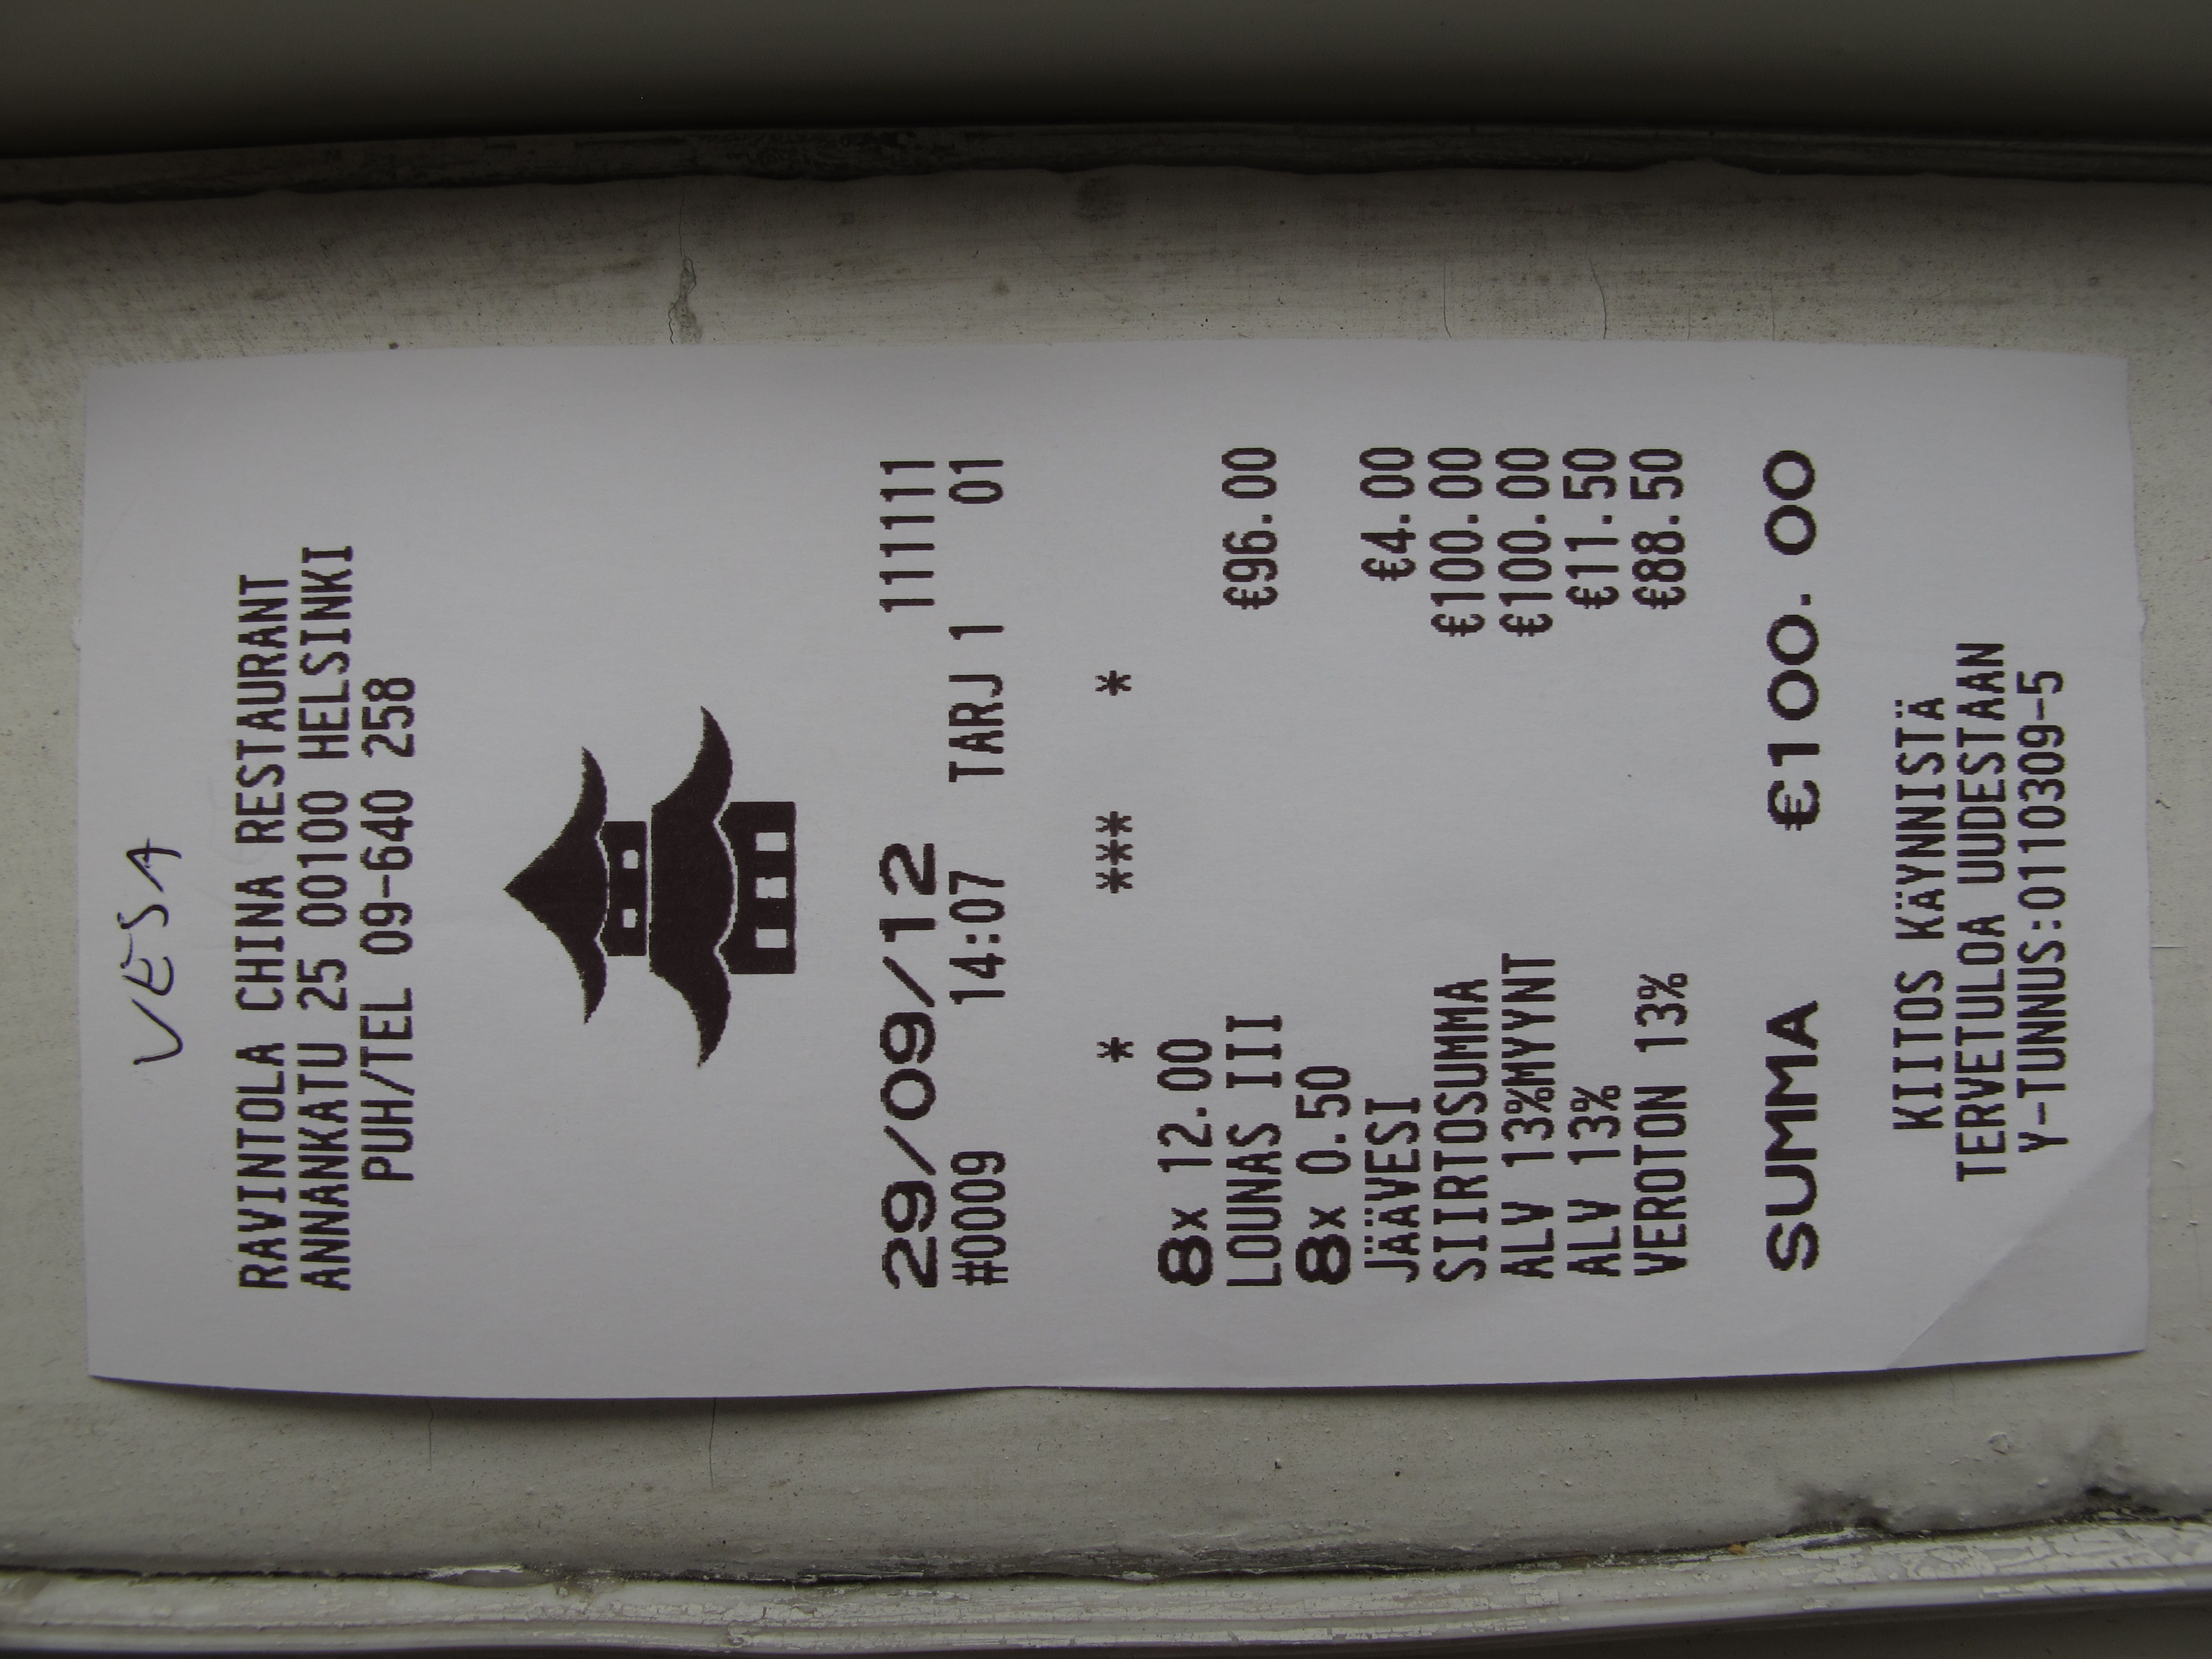
\includegraphics[width=80mm, angle=270]{pictures/alv-kuitti}
    \begin{vastaus}
         $13\,\%$ sadasta eurosta on $13$ euroa -- ei $11,50$ euroa, niin kuin kuitissa todetaan. Arvonlisävero lasketaan suhteessa verottomaan hintaan, ei lopulliseen myyntihintaan.
    \end{vastaus}
\end{tehtava}

\begin{tehtava} %tällaisesta esimerkkiä
Eräällä luentokurssilla on $44$ tunnin mittaista luentoa. Kurssin hyväksyttävään suoritukseen opiskelijan tulee olla läsnä vähintään $80$ prosentilla luennoista. Kuinka monelle luennolla opiskelija voi jättää menemättä niin, että kurssin saa vielä suoritettua?
	\begin{vastaus}
	$8$ luentoa voi jättää väliin ($9$ on jo enemmän kuin $80$ prosenttia $44$:stä)
	\end{vastaus}
\end{tehtava}

\begin{tehtava}
\alakohdat{
    § Laukun normaalihinta on $225$ euroa, ja se on $25$ prosentin alennuksessa. Mikä on alennettu hinta?
    § Meijun kuukausipalkka on $1\,623,52$ euroa. Hän saa $1,3\,\%$ palkankorotuksen. Mikä on Jaakon kuukausipalkka korotuksen jälkeen?
    }
    \begin{vastaus}
    \alakohdat{
    § $168,75$ euroa
    § $1\,644,63$ euroa
    }
    \end{vastaus}
\end{tehtava}

\begin{tehtava}
Vuosien 2008 ja 2012 kunnallisvaaleissa ehdokkaita asettaneiden eduskunnan ulkopuolisten puolueiden saamat äänet koko maassa on esitetty seuraavassa taulukossa. Mukana ovat vain ne puolueet, jotka olivat mukana molemmissa vaaleissa. \\
\begin{tabular}{|c|c|c|}
\hline 
Puolue / Äänet & 2008 & 2012 \\ 
\hline
Itsenäisyyspuolue & $1\,482$ & $1\,303$ \\
\hline
\vtop{\hbox{\strut Kommunistinen}\hbox{\strut Työväenpuolue}}  & $1\,065$ & $704$ \\
\hline
Köyhien Asialla & $1\,059$ & $572$ \\ 
\hline
\begin{tabular}[x]{@{}c@{}}Suomen Kommunistinen\\Puolue\end{tabular} & $13\,986$ & $11\,174$ \\ 
\hline 
Suomen Työväenpuolue & $703$ & $538$ \\ 
\hline 
\end{tabular}
\alakohdat{
§ Minkä puolueen kannatus laski eniten äänissä laskettuna ja kuinka paljon?
§ Minkä puolueen ''äänisaalis'' laski eniten prosentuaalisesti (suhteellisesti) ja kuinka paljon?
}
	\begin{vastaus}
	\alakohdat{
	§ Suomen Kommunistisen Puolueen, $2\,812$ ääntä
	§ Köyhien Asialla -puolueen, $46$\,\%
	}
	\end{vastaus}
\end{tehtava}

\begin{tehtava}
    Piraattipuolueen kannatus oli vuoden 2011 eduskuntavaaleissa $0,5\,\%$ ja vuoden 2014 europarlamenttivaaleissa $0,7\,\%$.
    \alakohdat{
    § Kuinka monta prosenttiyksikköä kannatus kasvoi? (Tiedotusvälineissä kannatusmuutokset ilmoitetaan yleensä prosenttiyksiköissä.)
    § Kuinka monta prosenttia kannatus kasvoi?
    }
    \begin{vastaus}
        \alakohdat{
        § Kannatus kasvoi $0,2$ prosenttiyksikköä.
        § Kannatus kasvoi $40$ prosenttia.
        }
    \end{vastaus}
\end{tehtava}

\begin{tehtava}
    Samulin pituus on $165$\,cm ja Joonaksen $173$\,cm.
    \alakohdat{
        § Kuinka monta prosenttia Samulin pituus on Joonaksen pituudesta?
        § Kuinka monta prosenttia Joonaksen pituus on Samulin pituudesta?
        § Kuinka monta prosenttia Samuli on lyhyempi kuin Joonas?
        § Kuinka monta prosenttia Joonas on pidempi kuin Samuli?
    }
    \begin{vastaus}
        \alakohdat{
            § $95,4\,\%$
            § $104,8\,\%$
            § $4,62\,\%$
            § $4,85\,\%$
        }
    \end{vastaus}
\end{tehtava}

\begin{tehtava}
    Jalkapalloilija Georgios Samaras teki ensimmäisellä kaudellaan Skotlannin valioliigassa (2007--2008) $5$ maalia Celtic F.\,C.:n paidassa. Seuraavalla kaudella Samaras teki Celticille liigassa $15$ maalia. Kuinka monta prosenttia Samaraksen maalimäärä nousi?
    \begin{vastaus}
        $200\,\%$
    \end{vastaus}
\end{tehtava}

\begin{tehtava}
Vuosina 1983--1985 Pohjois-Amerikassa koettiin valtava videopelialan lama. Nintendo of American mukaan alan vuosittaiset tulot vuonna 1983 olivat vielä $3,2$ miljardia dollaria, mutta vuonna 1985 ne olivat pudonneet sataan miljoonaan dollariin. Kuinka monen prosentin laskusta on kyse?
	\begin{vastaus}
	Noin $97$ prosenttia
	\end{vastaus}
\end{tehtava}

\begin{tehtava}
Suomalaisista masennuspotilaista arviolta jopa $30$\,\%:lla on samanaikainen alkoholiongelma, ja alkoholista riippuvaisista arviolta jopa $60$\,\%:lla on kliinisesti merkittävä depressio.
	\alakohdat{
	§ Kuinka suuri osa masentuneista suomalaisista ei ole alkoholiongelmaisia (=alkoholiriippuvaisia)?
	§ Kuinka suuri osa alkoholiongelmaisista (=alkoholiriippuvaisista) suomalaisista ei ole masentuneita?
	§ Kumpia on suomalaisista enemmän: masentuneita vai alkoholiongelmaisia?
	}
	\begin{vastaus}
		\alakohdat{
	§ $70$\,\%
	§ $40$\,\%
	§ Masentuneita on enemmän. %esimerkkeihin Venn-digrammi!
	}
	\end{vastaus}
\end{tehtava}

\begin{tehtava} %selitä vero, ja kanta teoriaosuudessa
Tuotteen hinta koostuu sen verottomasta hinnasta ja tuotteesta maksettavasta arvonlisäverosta. Vuoden 2013 alusta Suomessa ruoan arvonlisäverokanta on ollut $14\,\%$. Mikä ruokakauppiaan tulee asettaa elintarvikkeensa verottomaksi hinnaksi, jos hän haluaa myyntihinnaksi houkuttelevalta näyttävän $9,99$ euroa?
	\begin{vastaus}
	Merkitään verotonta hintaa $x$:llä, jolloin saadaan yhtälö $x+0,14x=9,99\,€$, eli $1,14x=9,99\,€$, josta ratkeaa jakolaskulla $x=\frac{9,99\,€}{1,14}\approx 8,76\,€$. 
	\end{vastaus}
\end{tehtava}

\begin{tehtava}
Tutki, pitääkö seuraava päättely paikkansa: jos tuotteen myyntihinta on $p$ prosenttia suurempi kuin tuotteen veroton hinta, arvonlisäverokanta on $p$ prosenttia.
	\begin{vastaus}
	Pitää paikkansa
	 Tapa 1, ALV:n määritelmän ja prosenttikertoimen tulkinnan perusteella: Merkitään verotonta hintaa $x$:llä, jolloin myyntihinta saadaan arvonlisäveron määritelmän perusteella summasta $x+\frac{p}{100}x$. Tämä sievenee tuttuun muotoon $(1+\frac{p}{100})x$, josta nähdään, että verollinen myyntihinta on $p$ prosenttia suurempi kuin veroton hinta $x$. Koska myyntihinnan lauseke ja prosenttikertoimellinen lauseke ovat täsmälleen samat (vain eri muodossa), pitää väite paikkansa. Huomaa, että väite pitäisi paikkansa myös toisin päin: jos ALV-kanta on $p$ prosenttia, tuotteen myyntihinta on $p$ prosenttia suurempi kuin veroton hinta.
	
	Tapa 2, erotusprosentin avulla: Merkitään tuntematonta verotonta hintaa $x$:llä, tuntematonta verollista hintaa $y$:llä, ja kirjoitetaan erotusprosentin lauseke, jossa verrataan myyntihinnan ja verottoman hinnan erotusta verottomaan hintaan: $\frac{y-x}{x}$. Tästä pitäisi tulla väitteen mukaan $p$\,\%, eli saadaan yhtälö $\frac{y-x}{x}=\frac{p}{100}$.Ratkaistaan verollinen myyntihinta $y$: kertomalla yhtälö puolittain $x$:llä saadaan $y-x=\frac{p}{100}x$, ja lisäämällä puolittain $x$ saadaan $y=x+\frac{p}{100}x$ eli $y=(1+\frac{p}{100})x$. Prosenttikertoimesta nähdään, että $x$ on kasvanut $p$ prosentilla, eli verollinen myyntihinta on todellakin $p$ prosenttia suurempi kuin veroton hinta $x$.
	\end{vastaus}
\end{tehtava}

\begin{tehtava}
     Kirjan myyntihinta, joka sisältää arvonlisäveron, on $9\,\%$ suurempi kuin kirjan veroton hinta. Laske kirjan veroton hinta, kun myyntihinta on $27$ euroa.
    \begin{vastaus}
        Kirjan veroton hinta on $24,77$ euroa.
    \end{vastaus}
\end{tehtava}

\begin{tehtava}
    Vuonna 2012 yleinen arvonlisäveroprosentti Suomessa oli $23\,\%$ tuotteen verottomasta hinnasta. Kuinka monta prosenttia arvonlisävero oli tuotteen myyntihinnasta?
    \begin{vastaus}
        $18,7\,\%$
    \end{vastaus}
\end{tehtava}

%\begin{tehtava}
%Marketta ottaa $1\,500$ pikavipin vuokrarästien maksamista varten.
%\end{tehtava}

\begin{tehtava}
\alakohdat{
§ Tuote A on $25$ prosentin alennuksessa ja maksaa tällöin yhtä paljon kuin tuote B, joka on parhaillaan $15$ prosentin alennuksessa. Kuinka monta prosenttia tuote A on B:tä kalliimpi?
§ Tuote C on $25$ prosentin alennuksessa ja maksaa tällöin yhtä paljon kuin tuote $D$, joka on parhaillaan $15$ prosentin alennuksessa ja maksaa tavallisesti $555$ euroa. Laske tuotteen C hinta.
}
	\begin{vastaus}
	\alakohdat{
	§ Merkataan $a$:lla tuotteen A hintaa ja $b$:llä tuotteen B hintaa. Annetuista tiedoista saadaan yhtälö $0,75a=0,85b$. $0,75$:llä jakamalla saadaan yhtälölle muoto $a=\frac{0,85}{0,75}b=\frac{17}{15}b \approx 1,133b$, josta voidaan lukea, että tuotteen A hinta on noin $13,3$ prosenttia suurempi kuin b:n. (Tarkka suhdeluku on $\frac{17}{15}$, mutta prosentit esitetään yleensä desimaalilukuina, ja tässä tapauksessa desimaalikehitelmässä toistuu numero 3 äärettömän pitkään, joten pyöristäminen on mielekästä. Alennusprosentit $25$ ja $15$ ovat kuitenkin tarkkoja, määrättyjä arvoja eivätkä arvioita, joten on turha puhua merkitsevistä numeroista tässä tapauksessa.)
	§ Saadaan yhtälö $0,75c=0,85\cdot 555\,€$, josta jakolaskulla vastaukseksi tulee $c=\frac{0,85\cdot 555\,€}{0,75}=629$ euroa.
	}
	\end{vastaus}
\end{tehtava}

\begin{tehtava}
Talletat pankkitilille $10\,000$ euroa, ja tilillä talletukselle kertyy korkoa $1,5$ prosenttia vuodessa. Alkutalletuksen jälkeen muita tilitapahtumia ei koronmaksun lisäksi ole. Tilillä oleva rahamäärä pyöristetään aina sentin tarkkuuteen.
\alakohdat{
§ Kuinka suuri ensimmäisen vuoden korko on?
§ Kuinka paljon rahaa tilillä on vuoden kuluttua?
§ Kuinka paljon rahaa tilillä on kymmenen vuoden kuluttua?
§ Kuinka paljon rahaa tilillä on $n$ vuoden kuluttua?
§ Kuinka monta prosenttia enemmän tilillä on rahaa $n$ vuoden kuluttua verrattuna alkuun?
}
	\begin{vastaus}
	 \alakohdat{
§ Korko on $1,5$\,\% talletuksesta, eli $0,015\cdot 10\,000\,€=150$ euroa.
§ $10\,000\,€+150\,€=10\,150\,€$ (tai $1,015\cdot 10\,000\,€=150\,€$)
§ $1,015^{10}\cdot 10\,000\,€\approx 11\,605,41\,€$
§ $1,015^n \cdot 10\,000$
§ $\frac{1,015^n \cdot 10\,000-10\,000}{10\,000}$, joka sievenee muotoon $1,015^n-1$ (vastaus ei siis riipu alkuperäisen talletuksen suuruudesta).
}
	\end{vastaus}
\end{tehtava}

\begin{tehtava}
    Erään pankin myöntämä opintolaina kasvaa korkoa $2\,\%$ vuodessa. Kuinka monta prosenttia laina on kasvanut korkoa alkuperäiseen verrattuna kymmenen vuoden kuluttua?
    \begin{vastaus}
        $22\,\%$
    \end{vastaus}
\end{tehtava}

\begin{tehtava}
    Sokerijuurikkaassa on $18\,\%$ sokeria. Kuinka paljon sokerijuurikkaita (tonneissa) tarvitaan valmistettaessa $8$ tonnia sokeriliuosta, jonka sokeripitoisuus on $4,5\,\%$?
    \begin{vastaus}
        $2$ tonnia
    \end{vastaus}
\end{tehtava}

\begin{tehtava} %esimerkki
    Hedelmissä on vettä aluksi $60\,\%$ niiden painosta. Kuinka monta prosenttia vedestä on haihdutettava, jotta hedelmissä tämän jälkeen olisi vain $20\,\%$ vettä?
    \begin{vastaus}
        $\approx83,3\,\%$ %pitää kertoa jossain, miten tuo ilmaisu luetaan...
    \end{vastaus}
\end{tehtava}

\begin{tehtava}
    (YO 2000K/4) Tuoreissa omenissa on vettä $80\,\%$ ja sokeria $4\,\%$. Kuinka monta prosenttia sokeria on samoissa omenissa, kun ne on kuivattu siten, että kosteusprosentti on $20$?
    \begin{vastaus}
        $16\,\%$
    \end{vastaus}
\end{tehtava}

\begin{tehtava}
    Kun matkalipun hintaa korotettiin $10,0\,\%$, matkustajien määrä väheni $10,0\,\%$. Kuinka monella prosentilla tällöin kasvoivat tai vähenivät liikennöitsijän lipputulot?
    \begin{vastaus}
        Lipputulot vähenivät $1$ prosentilla.
    \end{vastaus}
\end{tehtava}

\begin{tehtava}
    Iidan ja Matin duo saa julkisuutta, ja he alkavat myydä CD-levyään keikkojen yhteydessä $10$ euron kappalehinnalla. Jonkin ajan päästä he päättävät nostaa CD-levyn hintaa $20$ prosenttia. Matti alkaa kuitenkin katua päätöstä, ja ehdottaa tämän korotetun hinnan alentamista $20$ prosentilla, jotta useampi levy saataisiin myytyä.
    \alakohdat{
    § Mikä olisi tämän toimenpiteen jälkeen CD:n uusi hinta?
    § Montako prosenttia olisi alennuksen oltava, jotta oikeasti päästäisiin takaisin alkuperäiseen $10$ euron hintaan?
    }
    \begin{vastaus}
    \alakohdat{
    § Uusi hinta on $9,60$ euroa.
    § Vaadittava alennus on $17\,\%$.
    }
    \end{vastaus}
\end{tehtava}

\begin{tehtava}
    Askartelukaupassa on alennusviikot ja kaikki tavarat myydään $60\,\%$:n alennuksella. Viimeisenä päivänä kaikista hinnoista annetaan vielä lisäalennus, joka lasketaan aiemmin alennetusta hinnasta. Minkä suuruinen lisäalennus tulee antaa, jos lopullisen kokonaisalennuksen halutaan olevan $80\,\%$?
    \begin{vastaus}
        $50\,\%$
    \end{vastaus}
\end{tehtava}

\begin{tehtava} %esimerkiksi?
Oletetaan inflaation eli yksinkertaistettuna rahan arvon alenemisen olevan Suomessa eurojen tapauksessa vuosittain keskimäärin yksi prosentti. Talletusten ja sijoitusten arvo voi muuttua nimellisesti euroina, mutta kun myös inflaation vaikutus otetaan huomioon, puhutaan reaaliarvosta.
\alakohdat{
§ Kuinka korkeaa nettovuosikorkokantaa (eli lopullista korkoa, kun verot on otettu huomioon) pankin tulee vähintään tarjota, jotta asiakkaan talletuksen arvo oikeasti kasvaisi, kun inflaatio otetaan huomioon?
§ Millä nettovuosikorkokannalla talletuksen reaaliarvo kasvaa yhdellä prosentilla vuodessa?
}
	\begin{vastaus}
	\alakohdat{
	§ Olkoon alkuperäisen talletuksen suuruus $a$ ja pankin tarjoama korkokanta $p$\,\%. Jos sekä korko että inflaatio otetaan huomioon, talletuksen arvo on vuoden kuluttua $0,99(1+\frac{p}{100})a$. Jos prosenttikertoimet yhdessä sieventyvät suuremmaksi kuin $1$, talletuksen arvo kasvaa. Yhtälön $0,99(1+\frac{p}{100})=1$ ratkaisuna saadaan $p=\frac{100}{99}\approx1,01$. Jos siis korkokannaksi tarjotaan suurempaa kuin $p=\frac{100}{99}$\,\%, niin tällöin talletuksen reaaliarvo tulee kasvamaan.
	§ Saadaan yhtälö $0,99(1+\frac{p}{100})=1,01$, jonka ratkaisuna $p=\frac{200}{99}\approx 2,02$, eli tarjotun nettovuosikorkokannan tulee olla (sadasosien tarkkuudella niin kuin ne yleensä ilmoitetaan) $2,02$\,\%.
	}
	\end{vastaus}
\end{tehtava} %+Bitcoin-tehtävä

%http://www.paihdelinkki.fi/alkoholineuvonnan-opas/promille

\subsubsection*{Hallitse kokonaisuus}

\begin{tehtava}
Sekamehu valmistetaan sekoittamalla mehutiivistettä ja vettä suhteessa $1:5$. Jos mehutiiviste jo itsessään sisältää $50$\,\% vettä, kuinka monta prosenttia valmiista sekamehusta on vettä?
	\begin{vastaus}
	Kun sekoitetaan suhteessa $1:5$, mehussa on yhteensä kuusi ''osaa''. Näistä kuudesta osasta viisi on lisättyä vettä ja puolikas tiivisteen vettä. Vettä on siis viisi ja puoli osaa kuudesta. Veden osuus sekamehusta on siis $\frac{5+\frac{1}{2}}{6}=5,5/6\approx91,7\,\%$.
	\end{vastaus}
\end{tehtava}

\begin{tehtava}
Paranoidi perheenäiti ei ole opiskellut suuruusluokkia, ja hänellä menee millit ja mikrot sekaisin. Kuinka monta prosenttia liian suuren annoksen hän saa, kun hän syö ravintolisänä eräänä päivänä D-vitamiinia $50$ mikrogramman sijasta $50$ milligrammaa? (Vihje: älä yritä tätä kotona.)
	\begin{vastaus}
 Hän saa $999$ prosenttia liian suuren annoksen.
	\end{vastaus}
\end{tehtava}

\begin{tehtava} %esimerkki nopeudesta
Vuonna 1998 tanskalaisjohtoinen tutkimusryhmä onnistui sopivilla materiaalivalinnoilla hidastaamaan valoa sen tyhjiönopeudesta (\textit{täsmälleen} $299\,792\,458$ m/s, koska metri itsessään määritellään nykyään valonnopeuden avulla) $17$ metriin sekunnissa.
\alakohdat{
§ Kuinka monta prosenttia nopeus laski?
§ Kuinka monta prosenttia kauemmin hidastetulla valolla kestää ohittaa $100$ nanometrin kokoinen molekyyli?
§ Kuinka monta prosenttia kauemmin hidastetulla valolla kestää edetä matka $x$ (metriä)?
}
    \begin{vastaus}
\alakohdat{
§ Suhteellisen hyvälläkin tarkkuudella vastaus pyöristyy $100$\,\%:iin, mutta tämä ei tietenkään pidä kokeellisesti paikkaansa, koska valo ei pysähtynyt täysin. $17$\,m/s on luultavasti hyvin tarkka arvo, ja vastaukseksi sopii esimerkiksi $99,999994$\,\%. (Prosentit voivat olla hyvin köykäisiä käyttää, kun muutokset ovat monen suuruusluokan kokoisia. Kätevämpää voisi olla ilmoittaa vastaus esimerkiksi miljoonasosina sadasosien sijaan.)
§ Noin $1,76\cdot 10^9$\,\% %anna lauseke?
§ Noin $1,76\cdot 10^9$\,\%, eli sama kuin b-kohdassa. Matkan pituudella ei ole merkitystä, vaan $x$ supistuu muutosprosentin lausekkeesta pois: $\frac{\frac{x}{17}-\frac{x}{299\,792\,458}}{\frac{x}{299\,792\,458}}=\frac{299\,792\,458}{17}-1\approx1,76\cdot 10^7=1,76\cdot 10^9$\,\%.
}
    \end{vastaus}
\end{tehtava}

%kovalevytilan hävikkitehtävä

\begin{tehtava}
Eräällä kuvitteellisella saarella on vain kaksi valtiota: X ja Y. Valtioissa oli saman verran asukkaita, kunnes niiden välille syttyi sota. Tuhoisan ja hyvin yksipuolisen sodan seurauksena valtion Y asukasmäärä putosi sadasosaan entisestä, ja valtion X asukasmäärä putosi viisi prosenttia.
\alakohdat{
§ Esitä kokonaislukujen suhteena valtioiden sodan jälkeiset asukasmäärät.
§ Kuinka monta prosenttia valtion Y sodanjälkeinen asukasmäärä on koko saaren sodanjälkeisestä asukasmäärästä? Anna vastaus prosentin sadasosien tarkkuudella.
§ Kuinka monta prosenttia saaren asukasmäärä väheni sodan seurauksena?
}
	\begin{vastaus}
	\alakohdat{
	§ $95:1$
	§ $1,04\,\%$
	§ Olkoon $a$ valtion X tai Y alkuperäinen populaatio (sama molemmissa), jolloin saaren alkuperäinen populaatio on $2a$. Uusi asukasmäärä on $0,01\cdot a+0,95\cdot a$. Laskemalla vanhan ja uuden saaripopulaation erotus verrattuna alkuperäiseen saadaan: $\frac{2a-(0,01\cdot a+0,95\cdot a)}{2a}=\frac{2a-0,01a-0,95a}{2a}=\frac{1,04a}{2a}=\frac{1,04}{2}=0,52=52\,\%$. (Voi toki myös laskea vain uuden ja vanhan suhteen ja päätellä siitä tuloksen.)
	}
	\end{vastaus}
\end{tehtava}

\begin{tehtava}
	Avoin kierros laserhippaa (laser tag) maksaa yhdeltä pelaajalta $9$ euroa. Pelialueen voi kuitenkin varata seurueelle hintaan $260$ euroa. Mette on menossa pelaamaan viiden kaverinsa kanssa. 
	\alakohdat{
		§ Kuinka monta prosenttia kalliimpaa on varata joukolle yksityispeli kuin liput avoimeen peliin?
		§ Kuinka suuri seurueen on vähintään oltava, jotta yksityispeli tulisi halvemmaksi?
	}
	\begin{vastaus}
		\alakohdat{
			§ $381\,\%$
			§ $29$
		}
	\end{vastaus}
\end{tehtava}

\begin{tehtava}
Jos geenitekniikan laboratoriossa käsitellään tai tutkitaan RNA:ta, täytyy kyseistä DNA:n sukulaismolekyyliä tuhoavat entsyymit deaktivoida. Dietyylipyrokarbonaatti (DEPC) on voimakas proteiineja denaturoiva ja sakkaava yhdiste, ja sopii tähän tarkoitukseen hyvin. Tavallinen ohje tarvittavan puhdistusliuoksen valmistamiseen on, että valmista $100$ prosentin DEPC-liuosta laimennetaan $94$-prosenttisella etanolilla $10$-prosenttiseksi. Etanoli on laimennettu puhtaalla vedellä. Kuinka paljon vettä on $500$ millilitrassa valmista käyttöliuosta? Jokainen ilmoitettu prosentuaalinen arvo on \termi{tilavuusprosentti}{tilavuusprosentti} eli kunkin komponentin tilavuuden suhde koko liuoksen tilavuuteen.
	\begin{vastaus}
	Valmiista liuoksesta $10\,$\% on DEPC:tä ja $90\,$\% laimennettua etanolia, josta $94\,$\% on etanolia ja $6$\,\% vettä. Vettä on siis $0,06\cdot0,90\cdot500$\,ml$=27$\,ml.
	\end{vastaus}
\end{tehtava}

%Lisännyt Aleksi Sipola 10.11.2013
\begin{tehtava}
    (YO 1991K/5a) Luvun $\sqrt{r^2-a^2}$ likiarvona voidaan käyttää lukua $r-{\frac{1}{2}a^2}/r$. Laske tämän nojalla $\sqrt{3}$ likiarvo sopivia kokonaislukuja $r$ ja $a$ käyttäen. Kuinka monta prosenttia tämä likiarvo poikkeaa tarkasta arvosta?
    \begin{vastaus}
    Kun $r=2$ ja $a=1$, saadaan kaavasta likiarvoksi tasan $1,75$. Koska $\sqrt{3}=1,732\ldots$, likiarvo poikkeaa noin $1,04\,\%$.
    \end{vastaus}
\end{tehtava}

\subsubsection*{Lisää tehtäviä}

%Kaksi suuryrityksellä on duopoli... yhteistulot 10 miljoonaa euroa, puoliksi. suuri markkinointikampanja, jolla voisi saada itselleen 80 prosenttia tuloista, maksaa 2,5 miljoonaa.

\begin{tehtava}
    (YO 1877/4) Kaupungissa tuli jokaisen talonomistajan suorittaa kaupungin kassaan $5\,\%$ saadusta hyyrymäärästä [vuokrasta, ruotsin sanasta \textit{hyra}]. Sittemmin määrättiin, että mainittu prosentti oli oleva $10$. Monellako prosentilla talonomistajien täytyi korottaa hyyryjä saadakseen saman puhtaan säästön kuin ennen?
    \begin{vastaus}
        $5,6\,\%$
    \end{vastaus}
\end{tehtava}
	
\begin{tehtava}
Miksi ei kannata mennä ostoksille kauppaan, joka mainostaa liikkeessä olevan ''$-40$\,\%:n alennus''?
	\begin{vastaus}
	Pelkkä ''$40$ prosentin alennus'' tarkoittaa, että hinnat on kerrottu prosenttikertoimella $1-\frac{40}{100}=0,6$. Jos kyseessä on negatiivinen alennus, prosenttikerroin on $1-\frac{-40}{100}=1+\frac{40}{100}=1,4$, eli hintoja on kasvatettu!!!!11
	\end{vastaus}
\end{tehtava}

\begin{tehtava} 
		$\star$ Postapokalyptisessa Turussa ihmiset asuvat luolissa. Eräässä luolassa asuu $99$ ihmistä. Aikuisia on $50\,\%$ vähemmän kuin lapsia. Montako aikuista luolassa asuu?
	\begin{vastaus}
	Luolassa asuu $33$ aikuista.
	\end{vastaus}
\end{tehtava} % jonnekin tehtävään toisaalta poistettu "ilman ongelmia tai todistuksen yleisyyden heikentymistä (''\textit{without loss of generality}'', \textit{WLOG})"

\end{tehtavasivu}